\begin{frame}{Causal Analysis}
Suppose we have a new drug we want to test to see how efficacious it is.
 \begin{itemize}
  \item We would like to be able to say ``The drug leads to better health''
  \begin{itemize}
   \item But need an RCT to say this
   \begin{itemize}
    \item Randomization minimizes differences between groups at baseline
   \end{itemize}

   \item We only have observational data
   \item Thus differences could be attributed to the drug or confounding
   
   \begin{itemize}
    \item e.g. healthier people were much more likely to take the drug at baseline
   \end{itemize}

  \end{itemize}
Idea: Try to balance the covariates to reduce the effects of confounding
so the two groups seem identical at baseline
 \end{itemize}

\end{frame}

\begin{frame}{Counterfactual Model}
\begin{itemize}
 \item Suppose that for or every person, there are two potential outcomes
 \begin{itemize}
  \item $Y_i(0)$ - The outcome if they had taken the control, $Z=0$
  \item $Y_i(1)$ - The outcome if they had taken the treatment, $Z=1$
 \end{itemize}
\item Obviously, we only observe one. \textit{The fundamental problem of causal inference}
\item If we could observe both, then we could observe the causal effects for each person
\item Estimands of interest:
\begin{itemize}
 \item Average Treatment Effect (ATE) $E[Y_i(1)-Y_i(0)]$. The effect of moving entire population
 from treated to untreated
 \item Average treatment effect for the treated (ATT) $E[Y_i(1)-Y_i(0)|Z=1]$. The average treatment
 effect for those actually treated
\end{itemize}
\item In survival, the ATE is the difference in survival time
\end{itemize}
 
\end{frame}

\begin{frame}{Propensity scores}
\begin{block}{Definition}
The propensity score is the probability that the subject received the treatment given the subjects \textit{pretreatment}
covariates. It is computed using the patient's baseline (pretreatment) information \cite{Rosenbaum1983}
\end{block}
 \begin{itemize}
  \item Defined as  $e_i(x)=P(Z_i =1 |X_i)$
  \item Assume that the covariates play a role in how the subject chose treatment
  \item If we assume that $(Y(0),Y(1))\perp T|X \implies (Y(0),Y(1))\perp T|e(X)$
  \item Controlling for propensity score will make groups seem indistinguishable
  \item Thus, we may treat it as if it were an RCT
 \end{itemize}

\end{frame}

\begin{frame}{Common Propensity Score Methods}
\begin{itemize}
 \item Matching: Match treatment and controls on their propensity score, calculate ATE
 \item Stratification: Stratify on propensity score, weight and combine ATE in each stratum
 \item Weighting: Weight each observation by the inverse of its propensity score, and then calculate ATE
 
  \begin{figure}[h!]
  \centering
    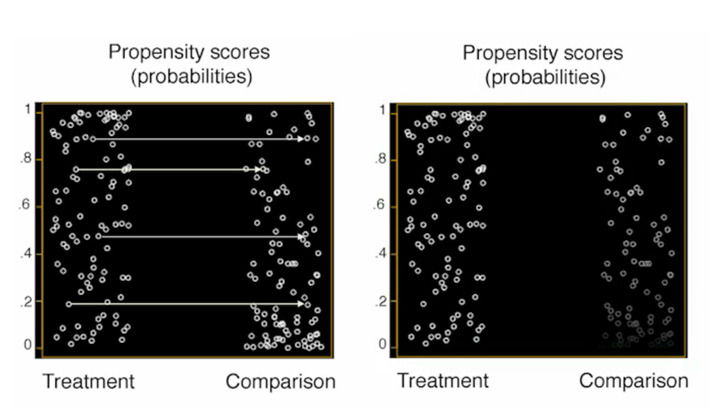
\includegraphics[width=0.8\textwidth]{ps_examples.png}
    \caption{Taken from TWANG shortcourse \cite{Rand2015}}
\label{fig:psexamp}

\end{figure}
\end{itemize}


\end{frame}

\begin{frame}{Propensity Score Issues}
 \begin{itemize}
  \item Unmeasured confounders
  \item Choice of pretreatment covariates in the propensity score model
  \item Different models and methods may lead to different conclusions
 \end{itemize}

\end{frame}
